\documentclass{article}
\usepackage{amsthm}
% \usepackage{ntheorem}
\usepackage{amsfonts}
\usepackage{graphicx}

% define break theorem style
\newtheoremstyle{break}
  {\topsep}{\topsep}%
  % {\itshape}{}%
  {\normalfont}{}%
  {\bfseries}{}%
  {\newline}{}%

% define definition 
\theoremstyle{break}
\newtheorem{definition}{Definition}[subsection]

\newcommand*{\Z}{\mathbb{Z}}
\newcommand*{\N}{\mathbb{N}}

\begin{document}
\title{Definitions for Abstract Algebra}
\author{Riley Weber}
\maketitle

Taken from \underline{Abstract Algebra: An Introduction} by Thomas W.
Hungerford (ISBN 978-1111569624). Created to study while taking MATH 3163:
Modern Algebra at UNC Charlotte. Definitions are ordered as they are in the
book and sectioned by chapter.

\section{Arithmetic in $\Z$ Revisited}
\subsection{}

\begin{definition}[Well-Ordering Axiom] 
  every non-empty subset of the set of non-negative integers has a least 
  element
\end{definition}

\subsection{}
\begin{definition}[Divisibility]
  Let $a, b \in \Z$ with $b \neq 0$. We say that $b$ divides $a$ and
  write $b \mid a$ if $a=bc$ for some $c \in \Z$.
\end{definition}

\begin{definition}[Greatest Common Divisor]
  Let $a, b \in \Z$, not both zero. The greatest common divisor ($gcd$) is
  the greatest integer that divides both $a$ and $b$. This means that if $d$ is
  the $gcd$ of $a$ and $b$, then
  \begin{enumerate}
    \item $d \mid a$ and $d \mid b$
    \item if $c \mid a$ and $c \mid b$, then $c \leq d$
  \end{enumerate}
  The greatest common divisor is often written $d = gcd(a,b)$ or simply
  $(a,b)$. it is also frequently called the greatest common \emph{denominator}.
\end{definition}

\subsection{}
\begin{definition}[Primality]
  An integer $p$ is said to be \textbf{prime} if $p \neq 0, \pm 1$ and the
  only divisors of $p$ are $\pm 1$ and $\pm p$.
\end{definition}

\section{Congruence in $\Z$ and Modular Arithmetic}
\subsection{}
\begin{definition}[Congruence Modulo $n$]
  Let $a, b, n \in \Z$ and $n > 0$. We say $a$ is congruent to $b$ modulo $n$
  and write $a \equiv b (mod n)$ if $n \mid a - b$.
\end{definition}

\begin{definition}[Congruence Class]
  Let $a, n \in \Z$ and $n > 0$. The congruence class of $a$ modulo $n$
  (written $[a]_n$ or $[a]$) is the set of all integers that are congruent to
  to $a$ modulo $n$. That is, $[a] = \{b | b \in \Z$ and $b \equiv a (mod n)\}$
\end{definition}

\begin{definition}[The Set of All Congruence Classes] 
  $\Z_n$, read "$\Z$ mod $n$" is the set of all congruence classes modulo n.
  Note that for every $n$ where $n \in \Z$ and $n > 1$, $\Z_n$ is a finite set,
  but each congruence class in that set is an infinite set. 
\end{definition}

\subsection{}
\begin{definition}[Addition and Multiplication in $\Z_n$]
  $[a] \oplus [b] = [a + b]$
  \\$[a] \odot [b] = [a \cdot b]$
\end{definition}

\subsection{}
\begin{definition}[Unit]
  Let $n \in \N$. A member of $\Z_n$ is a \textbf{unit} of $\Z_n$ if the
  equation $a \odot x = [1]$ has a solution in $\Z_n$. In this case, the
  element $x$ is called the \textbf{multiplicative inverse} and is denoted 
  $a^{-1}$
\end{definition}

\pagebreak
\section{Rings}

\subsection{}

\begin{definition}[Ring]
  A ring is a nonempty set $R$ equipped with two operations (usually written as
  addition and multiplication) that satisfy the following axioms.

  For all $a, b, c \in R$:

  \renewcommand{\arraystretch}{1.5}
  \begin{tabular}{l p{6cm} p{4cm}}
    1. & If $a \in R$ and $b \in R$, then $a + b \in R$ & [Closure for
    addition] \\

    2. & $a + (b + c) = (a + b) + c$ & [Associative addition] \\

    3. & $a + b = b + a$ & [Commutative addition] \\

    4. & There is an element $0_R \in R$ such that $a + 0_R = a = 0_R + a$ for
    every $a \in R$ & [Additive identity or zero element] \\

    5. & For each $a \in R$, the equation $a+x=0_R$ has a solution in R &
    [Additive inverse] \\

    6. & If $a \in R$ and $b \in R$, then $ab \in R$ & [Closure for
    multiplication] \\

    7. & $a(bc) = (ab)c$ & [Associative multiplication] \\

    8. & $a(b + c) = ab + ac$ and $(a + b )c = ac + bc$ & [Distributive laws]
    \\
  \end{tabular}
\end{definition}

\begin{definition}[Commutative Ring]
  A commutative ring is a ring $R$ in which $ab = ba$ for all $a, b \in R$
  (commutative multiplication).
\end{definition}

\begin{definition}[Ring with Identity] A ring with identity is a ring $R$ that
  contains a special element $1_R$ such that $a \cdot 1_R = a = 1_R \cdot a$
  for all $a \in R$ (multiplicative identity).
\end{definition}

\begin{definition}[Integral Domains]
  An integral domain is a commutative ring $R$ with identity such that if $a, b
  \in R$ and $ab = 0_R$ then either $a = 0_R$ or $b = 0_R$.
\end{definition}

\begin{definition}[Field]
  A field is a commutative ring $R$ with identity $1_R$ such that if $a \in R
  \setminus \{0_R\}$ then $a$ is a unit (i.e. the equation $ax = 1_R$ has a
  solution in $R$)
\end{definition}

Following is a diagram which illustrates what common sets are also rings,
fields, and the like.

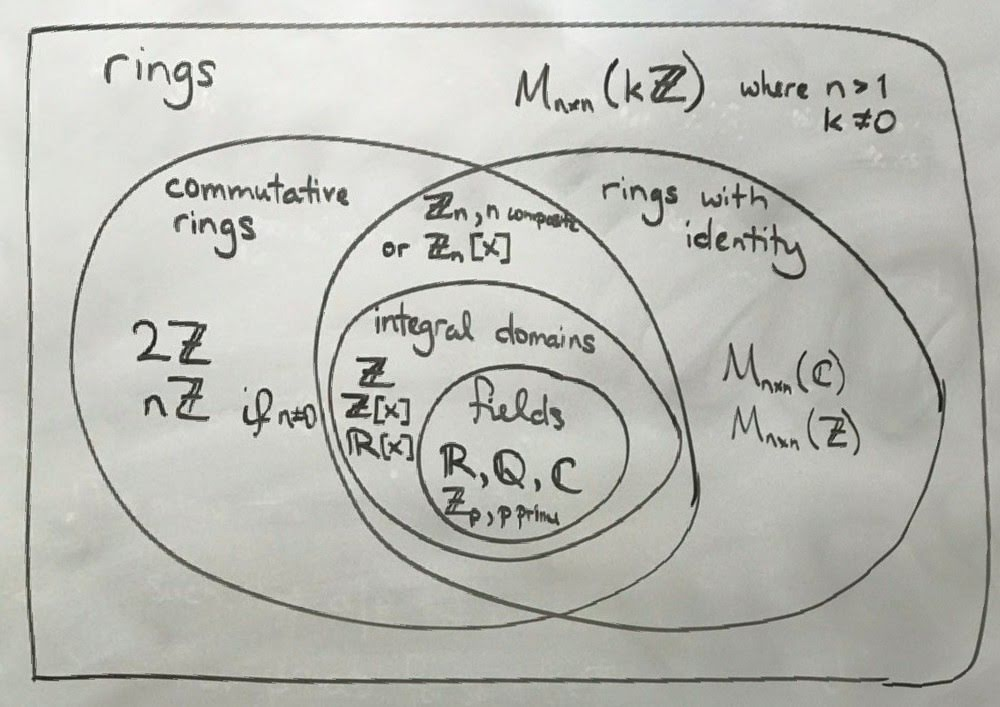
\includegraphics[width=\linewidth]{ring-venn-diagram.jpg}

\section{Arithmetic in $F[x]$}
\subsection{Polynomial Arithmetic and the Division Algorithm}

\begin{definition}[Polynomials]
  \textit{Note: this "definition" is listed as theorem 4.1 in the book. 
  However, since it is assumed in the text and honestly it defines what it
  means to be a polynomial, it has been included here.}

  Suppose $R$ is a ring. Then, $R[x]$ is the ring of polynomials with
  coefficients in $R$; i.e., $R[x] = R \cup \{r_0 + r_1 x + r_2 x^2 + ... + r_n
  x^n : r_0, ..., r_n \in R$ and $r_n \neq 0_R \}$

  Here $x$ is just a letter. Also, notice that saying $R[x] = R \cup \{ r_0 +
  r_1 x + r_2 x^2 + ... + r_n \}$ is redundant. The content of the curly
  braces includes $R$, because $R$ is the special case of $R[x]$ where all
  coefficients except $r_0$ are $0_R$. It is included in this definition for
  emphasis only.

  Observations:
  \begin{itemize}
    \item $R$ is a subring of $R[x]$
    \item The members of $R$ are called the "constant polynomials" in $R[x]$. 
  \end{itemize}
\end{definition}

\begin{definition}[Polynomial Arithmetic]
  If $f(x), g(x) \in R[x]$, then $+$ and $\cdot$ are defined in the "usual"
  way. I.e.:

  \begin{itemize}
    \item $(r_0 + r_1x + r_2x^2 + ... + r_nx^n) + (s_0 + s_1x + s_2x^2 + ... +
    s_mx^m) = (r_0 + s_0) + (r_1 + s_1)x + (r_2 + s_2)x^2 + ...$
    \item $(r_0 + r_1x + r_2x^2 + ... + r_nx^n) \cdot (s_0 + s_1x + s_2x^2 +
    ... + s_mx^m) = (r_0 \cdot s_0) + (r_0s_1 + r_1s_0)x + (r_0s_2 + r_1s_1 +rs_0
    +r_2s_0 s_2)x^2 + ...$
  \end{itemize}
\end{definition}

\begin{definition}[Degrees and Leading Coefficients]
  If $f(x) \in R[x] \setminus R$, then $f(x) = r_0 + r_1x + r_n x^n$ for some
  $n \in \N$ and $a_n \neq 0_R$. We say:

  \begin{itemize}
    \item $n$ is the \textbf{degree} of $f(x)$. This is often denoted
    "deg $f(x)$" or "deg$(f)$".
    \item $r_n$ is the \textbf{leading coefficient} of $f(x)$
  \end{itemize}

  There are a couple things to note about the degree of a polynomial:
  \begin{itemize}
    \item If $f(x) \in R \setminus \{ 0_R \}$, then the degree of $f(x)$ in
    $R[x]$ is $0$. Note that this means $f(x)$ have no variable terms, no $x$. 
    \item The degree of $0_R$ in $R[x]$ is undefined. $0_R$ does not have a
    degree. (But it can make sense to think of it as having degree $-\infty$)
  \end{itemize}
\end{definition}

\subsection{Divisibility in $F[x]$}

\begin{definition}[Divisibility and Factors]
  Let $F$ be a field and let $f(x), g(x) \in F[x]$ with $g(x) \neq 0_F$. We say
  that $g(x)$ \textbf{divides} $f(x)$ and that $g(x)$ is a \textbf{factor} of
  $f(x)$ if $f(x) = g(x)q(x)$ for some $q(x) \in F[x]$.
\end{definition}

\begin{definition}[Greatest Common Denominators for Polynomials]
  Let $F$ be a field and let $f(x), g(x) \in F[x]$ with at least one of them
  not equal to $0_F$. Then, the \textbf{greatest common divisor} of $f(x)$ and
  $g(x)$ is the unique, monic $d(x) \in F[x] \setminus \{0_F\}$ such that 
  \begin{enumerate}
    \item $d(x) \mid f(x)$ and $d(x) \mid g(x)$
    \item if $h(x) \mid f(x)$ and $h(x) \mid g(x)$ for some $h(x) \in F[x]$,
    then $deg(h) \leq deg(d)$
  \end{enumerate}
  This is often written as $d(x) = gcd(f(x), g(x))$
\end{definition}

\begin{definition}[Relative Primality]
  Let $F$ be a field and let $f(x), g(x) \in F[x]$, not both $0_F$. (read "$f$
  and $g$ are polynomials under the field $F$, not both zero). We say $f(x)$
  and $g(x)$ are \textbf{relatively prime} if $gcd(f(x), g(x)) = 1_F$
  \\ \\ For example:
  \begin{itemize}
    \item $gcd(x^2 - 1, x^2 + 2x + 1) = x + 1$, so these are \textbf{not}
    relatively prime 
    \item $gcd(x^2 - 1, x^3 + x) = 1$, so these \textbf{are} relatively prime
  \end{itemize}
\end{definition}

\subsection{Irreducibles and Unique Factorization}

\begin{definition}[Polynomial Associates]
  $f(x)$ is said to be an \textbf{associate} of $g(x)$ in $F[x]$ if and only if
  $f(x) = cg(x)$ for some nonzero $c \in F$.
  \\ \\ Notice that $c$ is in $F$ and not $F[x]$. This means that $c$ is constant.
\end{definition}

\begin{definition}[Irreducible Polynomials]
  Let $F$ be a field. A nonconstant polynomial $p(x) \in F[x]$ is said to be
  \textbf{irreducible} if its only divisors are its associates and the nonzero
  constant polynomials (units). A nonconstant polynomial that is not
  irreducible is said to be \textbf{reducible}.
  \\ \\ Notice that every polynomial of degree 1 in $F[x]$ is irreducible in $F[x]$
\end{definition}

\subsection{Polynomial Functions, Roots, and Reducibility}
Skipped because it is not on test 2

\subsection{Irreducibility in $Q[x]$}
Skipped because it is not on test 2

\subsection{Irreducibility in $R[x]$ and $C[x]$}
Skipped because it is not on test 2

\section{Congruence in $F[x]$ and Congruence-Class Arithmetic}

\subsection{Congruence and Congruence Classes in $F[x]$}

\begin{definition}[Congruence for Polynomials]
  Let $F$ be a field and $f(x), g(x), p(x) \in F[x]$ with $p(x)$ nonzero. Then
  $f(x)$ is \textbf{congruent to} $g(x)$ modulo $p(x)$ - written $f(x) \equiv
  g(x)($ mod $p(x))$ - provided that $p(x) \mid f(x) - g(x)$
  \\ \\ Recall that $\mid$ means "divides".
\end{definition}

\begin{definition}[Congruence Classes for Polynomials]
  Let $F$ be a field and $f(x), g(x), p(x) \in F[x]$ with $p(x)$ nonzero. The
  \textbf{congruence class} (a.k.a. \textbf{residue class}) of $f(x)$ modulo
  $p(x)$ is denoted $[f(x)]$ and consists of all polynomials in $F[x]$ that are
  congruent to $f(x)$ modulo $p(x)$. That is:
  \\ \\ $[f(x)] = \{ g(x) \mid g(x) \in F[x] $ and $ g(x) \equiv f(x) ($ mod
  $p(x)) \}$
\end{definition}

\begin{definition}[]
\end{definition}

\end{document}
